\chapter{Preliminaria matematyczne}\label{ch:02}

\section{Wprowadzenie}\label{sec:intromat}

Odwrócone wahadło to przykład obiektu robotycznego, który podczas normalnej pracy środek swojej masy ciężkości ma powyżej punktu obrotu, przez co jest układem wysoce niestabilnym. Układ taki charakteryzuje się dwoma punktami swobody:
\begin{itemize}
    \item punkt obrotu pręta
    \item poruszający się wzdłużnie wózek
\end{itemize} 
oraz tylko jednym wejściem sterującym:
\begin{itemize}
    \item prędkość wózka wzdłuż osi X.
\end{itemize}
Problem polega na znalezieniu takiego sterowania wózkiem, aby wahadło było utrzymane w osi pionowej, bez opadania w dół. Sterowanie odbywa się poprzez regulację prędkością wózka. \\

Jeżeli ruch jest opisany współrzędnymi uogólnionymi \(q=(q_1,q_2,...,q_n)^T\), które zdefiniowane są przez położenie liniowe i kątowe, oraz prędkościami uogólnionymi \(\dot{q}=(\dot{q}_1,\dot{q}_2,...,\dot{q}_n)^T \), które są pochodnymi położenia po czasie to lagranżian układu, który jest różnicą energii kinetycznej i potencjalnej można opisać wzorem:
\begin{equation}
    L(q,\dot(q))=K(q,\dot(q))-(q)
\end{equation}
Aby otrzymać równania ruchu układu, należy rozwiązać równania Eulera-Lagrange’a
\begin{equation}
    \frac{d}{dt}\frac{\partial  L}{\partial \dot{q}}-\frac{\partial L}{\partial q}=F,
\end{equation} gdzie \textit{F} to wszystkie siły niepotencjalne, takie jak:
\begin{itemize}
    \item siły tarcia,
    \item siły przyczepności,
    \item siły sterujące.
\end{itemize}
W przypadku, gdy żadne siły niepotencjalnie nie oddziaływują na układ podstawia się  \textit{F = 0} \cite{TchMu18}.

\section{Model matematyczny} \label{sec:modelmat}

Układ odwróconego wahadła został przedstawiony na rysunku \ref{fig:draw}. Rzeczywisty układ wahadła uwzględnia moment bezwładności pręta, który w tym modelu został zastąpiony przez pręt o pomijalnie małej masie i niewielkiej masie \textit{m} na jego końcu. 

\begin{figure}
    \centering
    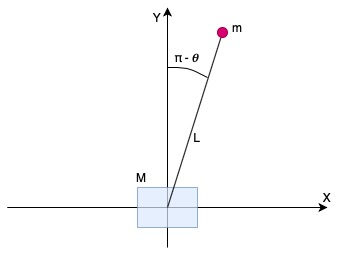
\includegraphics[scale=0.8]{praca_dyplomowa/figures/pendulum_draw.jpg}
    \caption{Układ odwróconego wahadła}
    \label{fig:draw}
\end{figure}

Współrzędne końca wahadła są opisane przez:
\begin{equation}
    \begin{cases}
    x_{p}=x+L\sin{\Theta}\\ 
    y_{p}=-L\cos{\Theta}
    \end{cases}
\end{equation}
gdzie \textit{x} to składowa położenia masy \textit{M}, wyznaczona przez rzut środka ciężkości na oś X układu. Składowe prędkości masy \textit{m} można wyznaczyć poprzez obliczenie pierwszych pochodnych po czasie jego współrzędnych pierwsze pochodne jego współrzędnych: 
\begin{equation}
    \begin{cases}
    \dot{x}_{p}=\dot{x}+L\dot{\Theta}\cos{\Theta}\\
    \dot{y}_{p}=L\dot{\Theta}\sin{\Theta}
    \end{cases}
    \label{skladowe}
\end{equation}

Energię kinetyczną można przedstawić w postaci równania \ref{ekin}, przy założeniu, że ramię wahadła ma pomijalnie małą masę, a tym samym jego moment bezwładności jest równy 0.
\begin{equation}
    K=\frac{1}{2}M{v_{1}}^{2}+\frac{1}{2}m{v_{2}}^{2},
    \label{ekin}
\end{equation}
gdzie \textit{v\textsubscript{1}} i \textit{v\textsubscript{2}} to odpowiednio prędkości mas \textit{M} i \textit{m} i wynoszą:
\begin{equation}
    \begin{array}{l}
         v_1=\dot{x} \\
         v_2=\sqrt{{\dot{x}_p}^{2}+{\dot{y}_p}^{2}}
    \end{array}
\end{equation}
Korzystając z wyprowadzenia \ref{skladowe} kwadrat prędkość \textit{v\textsubscript{2}} można wyrazić następująco: 
\begin{equation}
    {v_2}^2=(\dot{x}+L\dot{\Theta}\cos{\Theta})^{2}+(L\dot{\Theta}\sin{\Theta})^{2}=\dot{x}^2+2L\dot{\Theta}\dot{x}\cos{\Theta}+L^2\dot{\Theta}^2,
\end{equation}
zatem energia kinetyczna układu jest równa:
\begin{equation}
    K=\frac{1}{2}(M+m)\dot{x}^2+mL\dot{\Theta}\dot{x}\cos{\Theta}+\frac{1}{2}mL^2\dot{\Theta}^2
\end{equation}

,,Energia potencjalna układu pochodzi od siły grawitacji działającej na kulę" \cite{TchMu18} i wyraża się wzorem:
\begin{equation}
    V=mgL\cos{\Theta}
\end{equation}

Łącząc wyprowadzone równania na energię kinetyczną i potencjalną otrzymamy lagranżian:

\begin{equation}
    L=K-V=\frac{1}{2}(M+m)\dot{x}^2+mL\dot{\Theta}\dot{x}\cos{\Theta}+\frac{1}{2}mL^2\dot{\Theta}^2-mgL\cos{\Theta}
\end{equation}

Do wyznaczenia równań Eulera-Lagrange’a potrzebne są następujące pochodne:
\begin{equation}
        \begin{array}{l}
         \frac{\partial L}{\partial x}=0 \\ \\
         \frac{\partial L}{\partial \Theta}=mg\sin{\Theta} \\ \\
         \frac{\partial L}{\partial \dot{x}}=(M+m)\dot{x}+mL\dot{\Theta}\cos{\Theta} \\ \\
         \frac{\partial L}{\partial \dot{\Theta}}=mL\dot{x}\cos{\Theta}+mL^2\dot{\Theta}
    \end{array}
    \label{pochodne}
\end{equation}

Obliczone pochodne \ref{pochodne} należy wykorzystać, aby otrzymać równania dynamiki:
\begin{equation}
    \label{rDyna}
    \begin{cases}
    \frac{d}{dt}\frac{\partial L}{\partial \dot{x}}-\frac{\partial L}{\partial x}= (M+m)\ddot{x}+mL\ddot{\Theta}\cos{\Theta}-mL\dot{\Theta}^2\sin{\Theta}=F-T \\
    \frac{d}{dt}\frac{\partial L}{\partial \dot{\Theta}}-\frac{\partial L}{\partial \Theta}=ml\ddot{x}\cos{\Theta}+mL^2\ddot{\Theta}-mgL\sin{\Theta},
    \end{cases}
\end{equation}
gdzie \textit{F} jest siłą sterująca, natomiast \textit{T} tarciem.